\documentclass[parskip=full]{scrartcl}
\usepackage[utf8]{inputenc}
\usepackage[T1]{fontenc}
\usepackage[ngerman]{babel}
\usepackage{enumerate}
\usepackage{enumitem}
\usepackage{hyperref}
\usepackage{graphicx}
\usepackage{float}
\usepackage{lmodern}
\usepackage{csquotes}
\usepackage[toc]{glossaries}

\setlist[enumerate]{itemsep=-2.5mm}
\setlist[enumerate,2]{label=\arabic*.}
\setlist[description]{itemsep=-2.5mm}
\newcommand{\req}[1]{\mbox{/#1/}}

\title{ContentBasedBrowser -CoBaB- \\ Pflichtenheft}
\hypersetup{
    colorlinks,
    citecolor=black,
    filecolor=black,
    linkcolor=black,
    urlcolor=black
}

\renewcommand{\glossarysection}[2][]{}
\makeglossaries
\newglossaryentry{Annotation}
{
name=Annotation,
description={ist ein in den Datensätzen vordefinierter Bereich eines Bildes oder Videos}
}

\newglossaryentry{Lesezeichen}
{
name=Lesezeichen,
description={ist ein Link für schnelleren Zugriff auf bestimmte, meist häufig besuchte Ergebnisse in einer Lesezeichen-Sammlung}
}

\newglossaryentry{Chronik}
{
name=Chronik,
description={ist eine Sammlung von gespeicherten zuletzt besuchten Seiten im Programm. \newline Wird als Synonym von Historie im Dokument verwendet}
}

\newglossaryentry{Feedback}
{
name=Feedback,
description={umfasst das Bewerten der generierten Ergebnisse und ihr Witerleiten an den Suchalgorithmen für eine verbesserte Suche}
}



\newglossaryentry{GUI}
{
name=GUI,
description={(engl. graphical user interface) Grafische Benutzeroberfläche}
}

\newglossaryentry{Dialog}
{
name=Dialog,
description={ist ein Element der grafischen Benutzeroberfläche, bei dem Eingaben vom Benutzer eingeholt werden}
}

\newglossaryentry{Versionsverwaltung}
{
name=Versionsverwaltung,
description={Versionsverwaltung ist ein System, dass Änderungen an Dateien erfasst und mit einem Zeitstempel dokumentiert, um beliebige vorherige Versionen wiederherzustellen. Der Gebrauch von Versionsverwaltung heißt Versionierung}
}

\newglossaryentry{Git}
{
name=Git,
description={ist eine freie Software zur Versionsverwaltung von Dateien}
}

\newglossaryentry{Phase}
{
name=Phase,
description={ist einer der Abschnitte im Verlauf der Entwicklung eines Softwareprodukts: Planung, Entwurf, Implementierung, Testen, Wartung und Pflege}
}

\newglossaryentry{Phasendokument}
{
name=Phasendokument,
description={ist das Resultat einer Phase der Softwareentwicklung}
}

\newglossaryentry{Qt}
{
name=Qt,
description={ist eine Klassenbibliothek, also eine Sammlung von Routinen und Hilfsmitteln in Form von Programmcode, die die Darstellung von grafischen Benutzeroberflächen erlaubt. Sie ist in der Programmiersprache C++ verfasst}
}

\newglossaryentry{Qt Creator}
{
name=Qt Creator,
description={ist eine integrierte Entwicklungsumgebung - ein Hilfsmittel bei der Erstellung von Programmcode}
}

\newglossaryentry{Qt Designer}
{
name=Qt Designer,
description={ist ein Hilfsmittel zum Entwerfen und Erstellen grafischer Benutzeroberflächen}
}

\newglossaryentry{Qt Test}
{
name=Qt Test,
description={ist eine Framework für Modultests - ein Hilfsmittel beim kontinuierlichen Testen eines Programms bereits während der Implementierung}
}

\newglossaryentry{Suchverfahren}
{
name=Suchverfahren,
description={ist eine Routine, die die Bilder bzw. Videos eines gegebenen Datensatzes in ihrer Ähnlichkeit mit einer gegebenen Suchvorlage bewertet. \newline Wird als Synonym von Suchalgorithmen im Dokument verwendet.}
}

\newglossaryentry{Widget}
{
name=Widget,
description={ist eine verallgemeinernde Bezeichnung für Komponenten eines GUI}
}

\newglossaryentry{Entwurfsmuster}
{
name=Entwurfsmuster,
description={ist eine Lösung für häufig auftretende Probleme beim Entwurf von Software}
}

\newglossaryentry{Model-View-Controller}
{
name=Model-View-Controller,
description={ist ein Muster zur Strukturierung von Software-Entwicklung in die drei Einheiten Datenmodell (engl. model), Präsentation (engl. view) und Programmsteuerung (engl. controller). Ziel des Musters ist ein flexibler Programmentwurf, der eine spätere Änderung oder Erweiterung erleichtert und eine Wiederverwendbarkeit der einzelnen Komponenten ermöglicht.}
}

\newglossaryentry{Doxygen}
{
name=Doxygen,
description={ist eine freie Software, die aus Quellcode und darin enthaltenen Kommentaren eine Softwaredokumentation erzeugt}
}


\begin{document}
\begin{titlepage}
\title{ContentBasedBrowser -CoBaB- \\ Implementierungsdokument}
\author{Anja Blechinger, Marie Bommersheim, Georgi Georgiev,\\ Tung Nguyen, Vincent Winkler, Violina Zhekova}
\date{März 2016}
\maketitle
\vspace{300pt}
\begin{tabular}{l l}
Projekt: & Media Browser zur inhaltsbasierten Suche in Bild- und Videodaten\\
Auftraggeber: & Arne Schumann,\\
 & Fraunhofer Institut für Optronik, Systemtechnik und Bildauswertung,\\
 & Karlsruhe\\
\end{tabular}
\thispagestyle{empty}
\end{titlepage}
\setcounter{page}{1}

\tableofcontents
\pagebreak

\section{Einleitung}
In diesem Dokument wird die Qualitätssicherung von CoBaB beschrieben. \newline
Die Aufgabe dieser Phase ist es, die Bedienbarkeit und Funktionalität von CoBaB zu testen und eventuelle Fehler zu beheben. Dies ermöglichen die im Pflichtenheft beschriebenen und weitere Testszenarien. \newline
Außerdem wird überprüft, wie viel des erarbeiteten Codes durch die Testfälle abgedeckt wird. 
\pagebreak

\section{Verwendete Tools}
Im Folgenden werden die für die Entwicklung von CoBaB verwendeten Tools vorgestellt.

\begin{itemize}
\item Qt Creator wurde als plattformunabhängige Entwicklungsumgebung für C++ verwendet.
\item Qt Designer wurde zur Erstellung der GUI - Elemente genutzt.
\item Automatisierte Komponententests wurden mit Hilfe von Qt Test durchgeführt.
\item Qt Linguist wurde für die Übersetzung der GUI ins Englische eingesetzt.
\item Zur Versionsverwaltung wurde Git verwendet.
\item Die Dokumentation des Quelltextes erfolgte über Doxygen auf Englisch.
\item Travis ermöglichte die kontinuierliche Systemintegration von CoBaB.
\item cppcheck diente zur statischen Codeanalyse.
\end{itemize}
\pagebreak

\section{Probleme}
\subsection{Projektstruktur}
Um Kompenententests nicht mit dem echten Produktcode zu vermengen wurde ein eigenes Qt-Projekt \enquote{test.pro}
angelegt, das nur Tests enthält und eine eigene ausführbare Datei erzeugt. Desweiteren wurde der Produktcode in zwei weitere Qt-Projekte unterteilt. Die \enquote{app.pro} enthält nur eine Quellcodedatei \enquote{main.cpp} und erzeugt als ausführbare Datei das fertige Produkt. Der verbleibende Quellcode stellt den Kern des Projekts dar und wird von \enquote{core.pro} umfasst. Erzeugt wird eine Bibliothek. Hierdurch wird ermöglicht den Kern statisch in die ausführbare Datei des Testprojekts zu binden. Auch in das ausführbare Produkt ist der Kern statisch gebunden.

\subsection{Pointer Ownership}
Durch die verwendung von C++14 (siehe Abschnitt 11.1 des Pflichtenhefts) ist die verwendung von unique\_ptr, die selbständig ihre Ziele löschen, möglich. Ebenso übernehmen einige Komponenten der Qt-Bibliothek den Besitz übergebene Zeiger. Dynamisch allokierte Objekte, die gleichzeitig von einem unique\_ptr und einer der besagen Qt-Komponenten besessen werden, könnten zwei Versuche das selbe Objekt zu löschen zur Folge haben. Dies ist undefiniertes verhalten. Es müssen beim Verwenden von unique\_ptr also mehrfache Löschungen beachtet werden.

\subsection{Logger}
Der verwendete Logger ist aus dem Artikel \enquote{A Lightweight Logger for C++} von Filip Janiszewski entnommen.
Dieser ist zu finden unter http://www.drdobbs.com/cpp/a-lightweight-logger-for-c/240147505.

\subsection{Move-Konstruktoren}
Die Verwendung von unique\_ptr in Komponenten, die beispielsweise durch Haltung von Instanzen in einem Container die Möglichkeit haben müssen verschoben (move) zu werden, macht die Implementierung eines Move-Konstruktors und eines Move-Zuweisungsoperators notwendig. In C++14 (im Speziellen C++11) ist die automatische Generierung solcher Funktionen vorgesehen, falls dies durch attributweise Durchführung möglich ist. Die auf der Plattform Windows verwendete Version 2013 des Visual Studio Compilers unterstützt dies jedoch nicht. (siehe https://msdn.microsoft.com/en-us/library/dn457344.aspx)
Komponenten die notwendigerweise Move unterstützen, enthalten daher manuell geschriebene Move-Konstruktoren und -Zuweisungsoperatoren. (zum Beispiel: PageRegistration)

\pagebreak

\section{Erweiterungen}
Dieser Abschnitt beschäftigt sich mit Erweiterungen, die während des Entwurfs und der Implementierung der Erstversion von CoBaB bedacht wurden.

\subsection{PageWidgets}
Die Benutzeroberfläche von CoBaB ist in sogenannte PageWidgets, von denen zu jeder Zeit genau eines angezeigt wird, zerteilt.
Daten, auf die von mehreren PageWidgets zugegriffen wird, werden über einen vom Navigator verwalteten Stack ausgetauscht.
Dadurch sind die PageWidgets im objektorientierten Sinne voneinander unabhängig, es können also Änderungen an einem PageWidget vorgenommen werden ohne dabei ein anderes zu betreffen.
Bei Änderungen ist jedoch zu beachten, dass ein aktives PageWidget bestimmte Daten in einer bestimmten Reihenfolge im Stack erwartet.
Unbedachte Änderungen an den Operationen, die den Stack betreffen, können die Funktionalität anderer PageWidgets beeinträchtigen.

Um ein neues PageWidget hinzuzufügen, muss zunächst ein neues Element in der Aufzählung PageType angelegt werden. Unter dieser wird ein neues PageWidget-Objekt in MainControl beim Navigator registriert. Um es anzuzeigen, muss es entweder beim Start des Navigators als initiales PageWidget angegeben werden oder es muss beim Navigator eine Transition, die das neue PageWidget als Ziel hat, registriert werden, damit es im Laufe des Programms eingeblendet wird. Auch hier ist zu beachten, dass PageWidgets, die auf das neue PageWidget folgen, den Stack in einem bestimmten Zustand erwarten.

\subsection{AnnotationDrawer}
Um Annotationen anderer Formen (z.B. Kreise, Ellipsen) anzeigen zu können, muss die neue Annotation von Annotation erben. Außerdem muss ein entsprechendes ClickableGraphicsItem erstellt werden, das von QGraphicsItem (z.B. QGraphicsEllipseItem) erbt. Um anklickbar zu sein, muss das Item das contextMenuEvent überschreiben und ein Signal mit der gewählten Annotation und der Mausposition aussenden. In Annotation muss die neue Form hinzugefügt werden und die fromStream Methode angepasst werden, um die richtige Annotation zu lesen. In der AnnotationGraphicsItemFactory muss, abhängig von der Form, das neue GraphicsItem erzeugt werden.

\subsection{Suchalgorithmen und Plugins}
Hinzufügen von Suchverfahren ist ein wesentliches Kriterium in der Entwicklung von CoBaB, weshalb Suchalgorithmen als Plugins implementiert werden. Qt bietet eine eigene API für das Umsetzen von Plugins und Plugin-Schnittstelle (man beachte hierzu auch die Qt-Dokumentation für Low-Level-Plugins). Ein neues CoBaB-Plugin umfasst ein Qt-Projekt, das neben den für Qt-Plugins notwendigen Einstellungen auch das CoBaB-Unterprojekt \enquote{interface} bindet. Dieses enthält eine Klasse, die das Plugin-Interface implementiert. Das Plugin-Interface wird duch die Klasse \enquote{Algorithm} angeboten. Es ist auch möglich eine der Unterklassen von \enquote{Algorithm}, die zusätzliche FUnktionen bieten, zu erben. (Man beachte die Dokumentation von \enquote{Algorithm} und den Unterklassen).
Auch Plugins die keine Suchalgorithmen implementieren sind denkbar und wurden im Entwurf bedacht. Sie verfügbar zu machen bedarf im Regelfall einer Anpassung in CoBaB selbst, jedoch keine Anpassung der Plugin-Schnittstelle.

\pagebreak

\section{Implementierte Anforderungen}
% !TeX spellcheck = de_DE_frami
\subsection{Pflichtanforderungen}
\begin{enumerate} [label=\bfseries /F \arabic*0/, leftmargin=*]
	\item DONE Starten des Programms
	\item DONE Beenden des Programms
	\item ? Automatisches Erkennen verfügbarer Suchverfahren
	\item DONE Übergeben eines Standardordners für die Bibliotheksdatensätze über die Kommandozeile
	\item DONE Anzeigen eines Hilfe-Dialogs mit Hinweisen zur Benutzung des Programms
	\item DONE Anzeigen eines About-Dialogs mit Informationen zum Programm
	\item DONE Rückkehr zur Bibliothek
	\newline
 
	\item DONE Anzeigen einer Bibliothek von Datensätzen
	\item DONE Auswählen eines Datensatzes, der nicht in der Bibliothek enthalten ist
	\item DONE Auswählen eines Datensatzes aus der Bibliothek
	\item DONE Anzeigen einer Übersicht der Bilder bzw. Videos des gewählten Datensatzes
	\item DONE Unterstützung der Bildformate JPEG, PNG und BMP
	\item DONE Anzeigen einer größeren Darstellung eines ausgewählten Bildes bzw. Videos des Datensatzes
	\item DONE Abspielen eines Videos aus Einzelbildern
	\item DONE Auswählen des vorherigen oder nächsten Bildes bzw. Videos für die große Ansicht
	\item DONE Auswählen eines Bildes bzw. Videos aus dem gewählten Datensatz als Suchvorlage
	\item DONE Anzeigen annotierter Bildbereiche
	\item DONE Auswahl eines annotierten Bildbereiches als Suchvorlage
	\item DONE Einschränkung der Suchvorlage auf einen benutzerdefinierten rechteckigen Bereich (falls keine Annotation gewählt wurde)
	\item DONE Auswahl eines für die gewählte Suchvorlage geeigneten Suchverfahrens
	\item DONE Anzeigen einer Beschreibung für die Suchverfahren
	\item ? Festlegen der für das gewählte Suchverfahren spezifischen Parameter
	\item DONE Anzeigen sämtlicher vorgenommener Einstellungen zur aktuellen Suche, um eine Überprüfung durch den Benutzer zu ermöglichen
	\item DONE Ändern beliebiger zu einer Suche vorgenommener Einstellungen
	\newline
	\item DONE Starten der Suche
	\item DONE Anzeigen einer Fortschrittsanimation während des Suchvorgangs
	\newline
	\item DONE Anzeigen einer sortierten Übersicht der Suchergebnisse
	\item DONE Optionales Einstellen eines Feedbacks zu einem Suchergebnis und Starten einer weiteren Suche mit diesem Feedback und dem selben Suchverfahren
	
	\item DONE Loggen von Informationen, Warnungen, Fehlern und Debugmeldungen
	 
\end{enumerate}

\subsection{Wunschanforderungen}
\begin{enumerate} [label=\bfseries /FW \arabic*0/, leftmargin=*]
	\item DONE Nicht-flüchtige Auswahl der Übersetzungen der GUI in Deutsch und Englisch
	\newline
	\item ? Wählen von mehreren Datensätzen, in denen gesucht wird
	\item DONE Generierung eines zufälligen oder festgelegten Vorschaubildes für den Datensatz
	\newline
	\item DONE Abspielen eines Benachrichtigungstons bei Abschluss einer Suche
	\item DONE Ein-/Abschalten des Benachrichtigungstons
	\item Abspielen von Videos aus Videodateien (mit Ausgabe der Audiospur)
	\newline
	\item Festlegung eines Wertes zwischen 0 und 10 als Feedback
	\item Durchführen einer weiteren Suche in den Ergebnissen einer bereits beendeten Suche mit anderem Suchverfahren
	\newline
	\item ? Wechsel in einen Vollbildmodus für Präsentation
	\item DONE Zoomen und Scrollen in der größeren Darstellung im Fotoanzeiger oder Videoplayer \label{fw:zoom_scroll}
	\item Anzeigen einer größeren Darstellung eines ausgewählten Suchergebnisses
	\newline
	\item DONE Nicht-flüchtiges Speichern der zuletzt verwendeten Datensätze
	\item Nicht-flüchtiges Speichern der Lesezeichen
	\item Automatisches nicht-flüchtiges Speichern der Suchchronik
	\item DONE Anzeigen der Historie der Datensätze
	\item Anzeigen einer Übersicht der Lesezeichen
	\item Anzeigen einer Übersicht der Suchchronik
	\item Wiederanzeigen der Ergebnisse eines Lesezeichens
	\item Wiederanzeigen der Ergebnisse der Suchchronik
	\newline
	\item Abbrechen der Suche mit Weiterführung der Oberfläche
\end{enumerate}
\pagebreak

\pagebreak

\section{Zeitplan}
\begin{figure}[H]
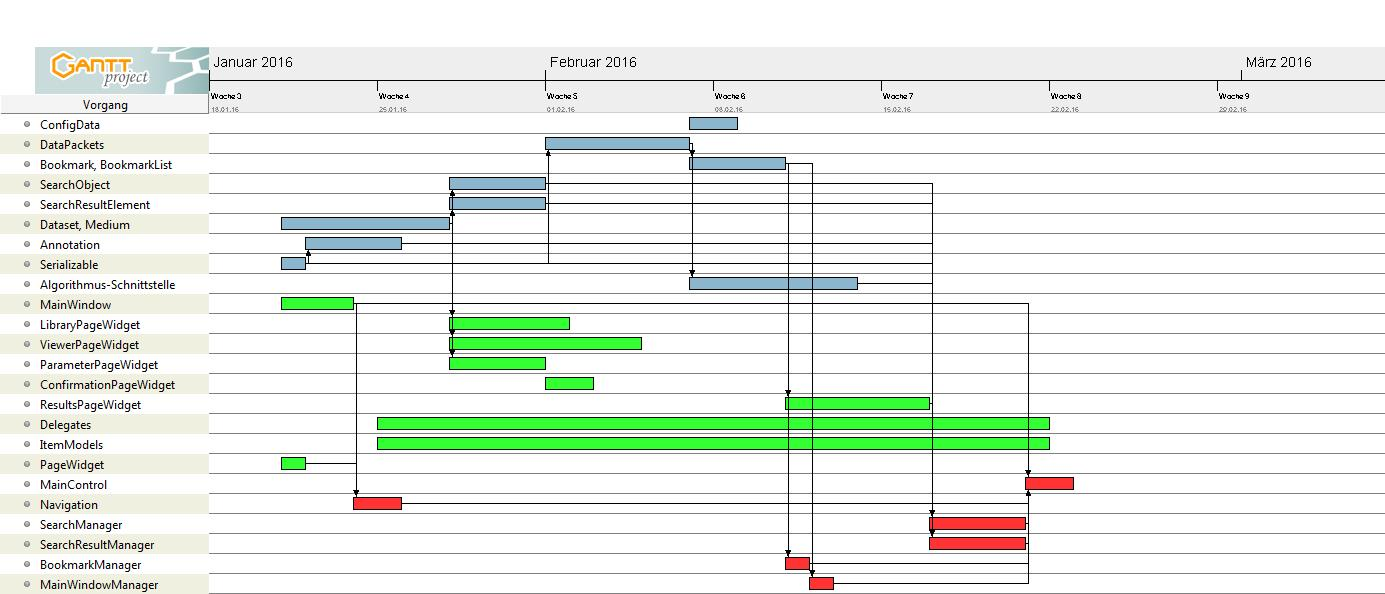
\includegraphics[width=18cm, height=13cm, angle = 90]{Zeitplan}
\caption{Implementierungszeitplan}
\end{figure}

Dieser Zeitplan wurde unmittelbar nach der Entwurfsphase erstellt. Hilfreich war diese Planung für die Reihenfolge, in der die Komponenten implementiert wurden. Allerdings haben die einzelnen Implementierungsschritte deutlich mehr Zeit in Anspruch genommen, als ursprünglich geplant war.
\pagebreak

\section{Unit Tests}
Folgende Klassen wurden mit Hilfe von Qt Test erfolgreich getestet:
\begin{itemize}
\item AlgorithmList
\item Annotation
\item Bookmark
\item BookmarkList
\item ConfigData
\item DataPacket
\item DatasetList
\item Dataset
\item Navigator
\item PageRegistration
\item PageStackFrame
\item RectangleAnnotation
\item SearchFeedback
\item SearchObject
\item SearchQuery
\item SearchResultElement
\item SearchResult
\item SingleFrameVideo
\end{itemize}
\pagebreak

\section{Glossar}
\printglossaries

\end{document}
